% Options for packages loaded elsewhere
\PassOptionsToPackage{unicode}{hyperref}
\PassOptionsToPackage{hyphens}{url}
%
\documentclass[
]{article}
\usepackage{amsmath,amssymb}
\usepackage{iftex}
\ifPDFTeX
  \usepackage[T1]{fontenc}
  \usepackage[utf8]{inputenc}
  \usepackage{textcomp} % provide euro and other symbols
\else % if luatex or xetex
  \usepackage{unicode-math} % this also loads fontspec
  \defaultfontfeatures{Scale=MatchLowercase}
  \defaultfontfeatures[\rmfamily]{Ligatures=TeX,Scale=1}
\fi
\usepackage{lmodern}
\ifPDFTeX\else
  % xetex/luatex font selection
    \setmainfont[]{NanumGothic}
    \setmonofont[]{UnShinmun}
\fi
% Use upquote if available, for straight quotes in verbatim environments
\IfFileExists{upquote.sty}{\usepackage{upquote}}{}
\IfFileExists{microtype.sty}{% use microtype if available
  \usepackage[]{microtype}
  \UseMicrotypeSet[protrusion]{basicmath} % disable protrusion for tt fonts
}{}
\makeatletter
\@ifundefined{KOMAClassName}{% if non-KOMA class
  \IfFileExists{parskip.sty}{%
    \usepackage{parskip}
  }{% else
    \setlength{\parindent}{0pt}
    \setlength{\parskip}{6pt plus 2pt minus 1pt}}
}{% if KOMA class
  \KOMAoptions{parskip=half}}
\makeatother
\usepackage{xcolor}
\usepackage[margin=1in]{geometry}
\usepackage{color}
\usepackage{fancyvrb}
\newcommand{\VerbBar}{|}
\newcommand{\VERB}{\Verb[commandchars=\\\{\}]}
\DefineVerbatimEnvironment{Highlighting}{Verbatim}{commandchars=\\\{\}}
% Add ',fontsize=\small' for more characters per line
\usepackage{framed}
\definecolor{shadecolor}{RGB}{248,248,248}
\newenvironment{Shaded}{\begin{snugshade}}{\end{snugshade}}
\newcommand{\AlertTok}[1]{\textcolor[rgb]{0.94,0.16,0.16}{#1}}
\newcommand{\AnnotationTok}[1]{\textcolor[rgb]{0.56,0.35,0.01}{\textbf{\textit{#1}}}}
\newcommand{\AttributeTok}[1]{\textcolor[rgb]{0.13,0.29,0.53}{#1}}
\newcommand{\BaseNTok}[1]{\textcolor[rgb]{0.00,0.00,0.81}{#1}}
\newcommand{\BuiltInTok}[1]{#1}
\newcommand{\CharTok}[1]{\textcolor[rgb]{0.31,0.60,0.02}{#1}}
\newcommand{\CommentTok}[1]{\textcolor[rgb]{0.56,0.35,0.01}{\textit{#1}}}
\newcommand{\CommentVarTok}[1]{\textcolor[rgb]{0.56,0.35,0.01}{\textbf{\textit{#1}}}}
\newcommand{\ConstantTok}[1]{\textcolor[rgb]{0.56,0.35,0.01}{#1}}
\newcommand{\ControlFlowTok}[1]{\textcolor[rgb]{0.13,0.29,0.53}{\textbf{#1}}}
\newcommand{\DataTypeTok}[1]{\textcolor[rgb]{0.13,0.29,0.53}{#1}}
\newcommand{\DecValTok}[1]{\textcolor[rgb]{0.00,0.00,0.81}{#1}}
\newcommand{\DocumentationTok}[1]{\textcolor[rgb]{0.56,0.35,0.01}{\textbf{\textit{#1}}}}
\newcommand{\ErrorTok}[1]{\textcolor[rgb]{0.64,0.00,0.00}{\textbf{#1}}}
\newcommand{\ExtensionTok}[1]{#1}
\newcommand{\FloatTok}[1]{\textcolor[rgb]{0.00,0.00,0.81}{#1}}
\newcommand{\FunctionTok}[1]{\textcolor[rgb]{0.13,0.29,0.53}{\textbf{#1}}}
\newcommand{\ImportTok}[1]{#1}
\newcommand{\InformationTok}[1]{\textcolor[rgb]{0.56,0.35,0.01}{\textbf{\textit{#1}}}}
\newcommand{\KeywordTok}[1]{\textcolor[rgb]{0.13,0.29,0.53}{\textbf{#1}}}
\newcommand{\NormalTok}[1]{#1}
\newcommand{\OperatorTok}[1]{\textcolor[rgb]{0.81,0.36,0.00}{\textbf{#1}}}
\newcommand{\OtherTok}[1]{\textcolor[rgb]{0.56,0.35,0.01}{#1}}
\newcommand{\PreprocessorTok}[1]{\textcolor[rgb]{0.56,0.35,0.01}{\textit{#1}}}
\newcommand{\RegionMarkerTok}[1]{#1}
\newcommand{\SpecialCharTok}[1]{\textcolor[rgb]{0.81,0.36,0.00}{\textbf{#1}}}
\newcommand{\SpecialStringTok}[1]{\textcolor[rgb]{0.31,0.60,0.02}{#1}}
\newcommand{\StringTok}[1]{\textcolor[rgb]{0.31,0.60,0.02}{#1}}
\newcommand{\VariableTok}[1]{\textcolor[rgb]{0.00,0.00,0.00}{#1}}
\newcommand{\VerbatimStringTok}[1]{\textcolor[rgb]{0.31,0.60,0.02}{#1}}
\newcommand{\WarningTok}[1]{\textcolor[rgb]{0.56,0.35,0.01}{\textbf{\textit{#1}}}}
\usepackage{graphicx}
\makeatletter
\def\maxwidth{\ifdim\Gin@nat@width>\linewidth\linewidth\else\Gin@nat@width\fi}
\def\maxheight{\ifdim\Gin@nat@height>\textheight\textheight\else\Gin@nat@height\fi}
\makeatother
% Scale images if necessary, so that they will not overflow the page
% margins by default, and it is still possible to overwrite the defaults
% using explicit options in \includegraphics[width, height, ...]{}
\setkeys{Gin}{width=\maxwidth,height=\maxheight,keepaspectratio}
% Set default figure placement to htbp
\makeatletter
\def\fps@figure{htbp}
\makeatother
\setlength{\emergencystretch}{3em} % prevent overfull lines
\providecommand{\tightlist}{%
  \setlength{\itemsep}{0pt}\setlength{\parskip}{0pt}}
\setcounter{secnumdepth}{-\maxdimen} % remove section numbering
\usepackage{fvextra}
\fvset{breaklines}
\ifLuaTeX
  \usepackage{selnolig}  % disable illegal ligatures
\fi
\usepackage{bookmark}
\IfFileExists{xurl.sty}{\usepackage{xurl}}{} % add URL line breaks if available
\urlstyle{same}
\hypersetup{
  pdftitle={multivariate\_lab\_hw2},
  pdfauthor={Na SeungChan},
  hidelinks,
  pdfcreator={LaTeX via pandoc}}

\title{multivariate\_lab\_hw2}
\author{Na SeungChan}
\date{2024-12-13}

\begin{document}
\maketitle

\begin{center}\rule{0.5\linewidth}{0.5pt}\end{center}

\section{1}\label{section}

Interpret the result of Box's M test. Can you assume equal covariance?

Box's M test의 H0는 공분산행렬이 동질적이라는 것이다. 즉 p-value가
유의수준 미만으로 나오면 귀무가설을 기각하여, 공분산행렬이 동질적이지
않고 그룹 간 차이가 있다고 결론을 내린다.

\begin{Shaded}
\begin{Highlighting}[]
\NormalTok{test\_varequal }\OtherTok{\textless{}{-}} \FunctionTok{BoxM}\NormalTok{(flea[,}\DecValTok{2}\SpecialCharTok{:}\DecValTok{7}\NormalTok{], }\AttributeTok{group =}\NormalTok{ flea}\SpecialCharTok{$}\NormalTok{species)}
\NormalTok{test\_varequal}\SpecialCharTok{$}\NormalTok{p.value}
\end{Highlighting}
\end{Shaded}

\begin{verbatim}
## [1] 0.2049986
\end{verbatim}

p.value = 0.2049986 \textgreater{} 0.05. flea beetles의 종에 따라
공분산행렬이 서로 다르다는 대립가설을 기각하지 못하며, 분산행렬이 서로
같다고 가정해도 될 것 같다. 이에 따라 MANOVA 등 모델을 사용할 수 있을
것이다.

\begin{center}\rule{0.5\linewidth}{0.5pt}\end{center}

\section{2}\label{section-1}

Box's M test assumes multivariate normality of each population. Is such
an assumption valid? Can we assume normality for each population? (See
Lab \#2)

\subsection{marginal normality : Q-Q plot for each
variable}\label{marginal-normality-q-q-plot-for-each-variable}

\begin{Shaded}
\begin{Highlighting}[]
\ControlFlowTok{for}\NormalTok{ (i }\ControlFlowTok{in} \DecValTok{2}\SpecialCharTok{:}\DecValTok{7}\NormalTok{) \{}
\NormalTok{  graph\_name }\OtherTok{\textless{}{-}} \FunctionTok{paste}\NormalTok{(}\StringTok{\textquotesingle{}Normal Q{-}Q Plot for\textquotesingle{}}\NormalTok{, }\FunctionTok{names}\NormalTok{(flea)[i])  }
  \FunctionTok{qqnorm}\NormalTok{(flea[,i], }\AttributeTok{main =}\NormalTok{ graph\_name)}
  \FunctionTok{qqline}\NormalTok{(flea[,i])}
\NormalTok{\}}
\end{Highlighting}
\end{Shaded}

\begin{center}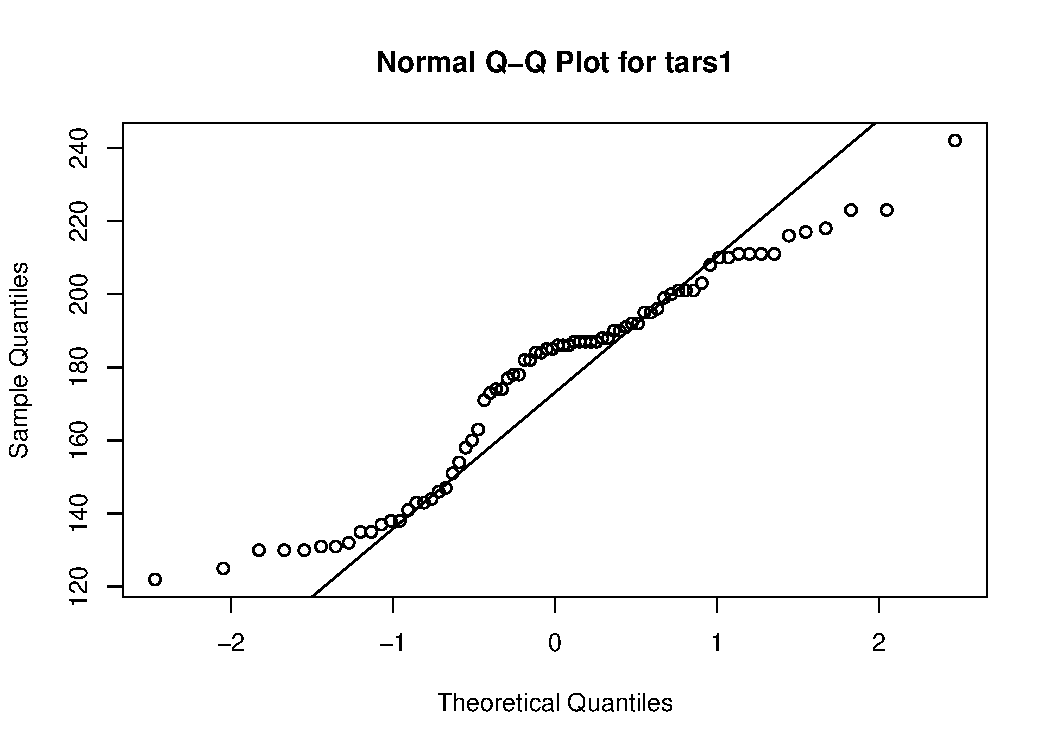
\includegraphics[width=0.8\linewidth]{multivariate_lab_hw2_files/figure-latex/unnamed-chunk-2-1} \end{center}

\begin{center}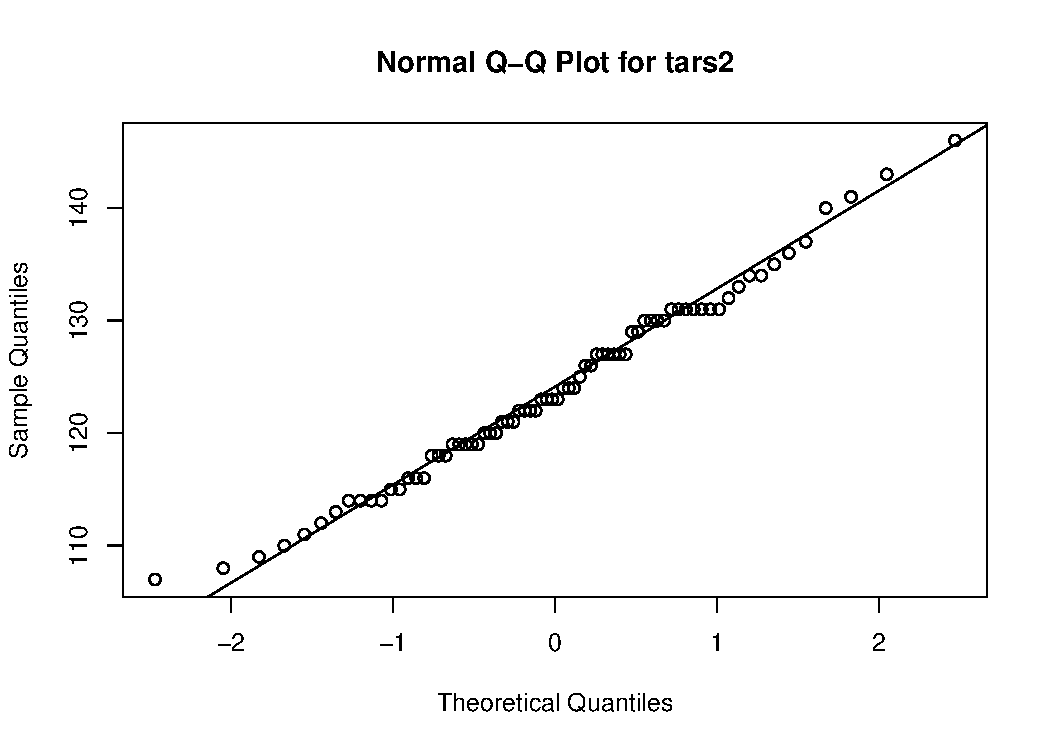
\includegraphics[width=0.8\linewidth]{multivariate_lab_hw2_files/figure-latex/unnamed-chunk-2-2} \end{center}

\begin{center}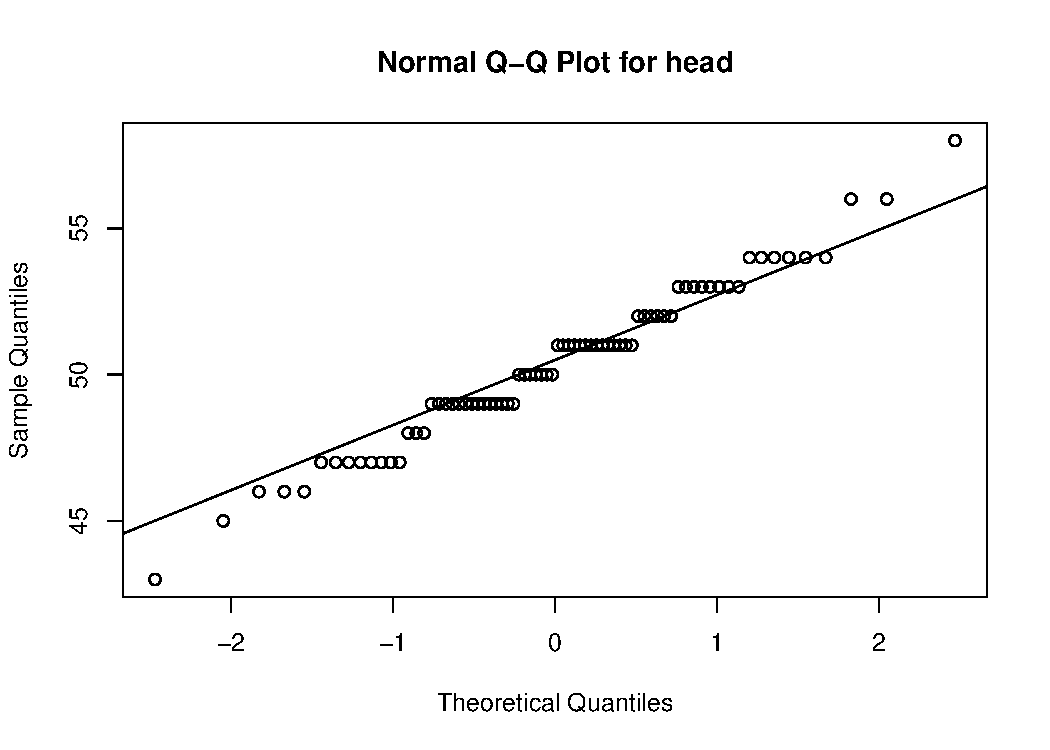
\includegraphics[width=0.8\linewidth]{multivariate_lab_hw2_files/figure-latex/unnamed-chunk-2-3} \end{center}

\begin{center}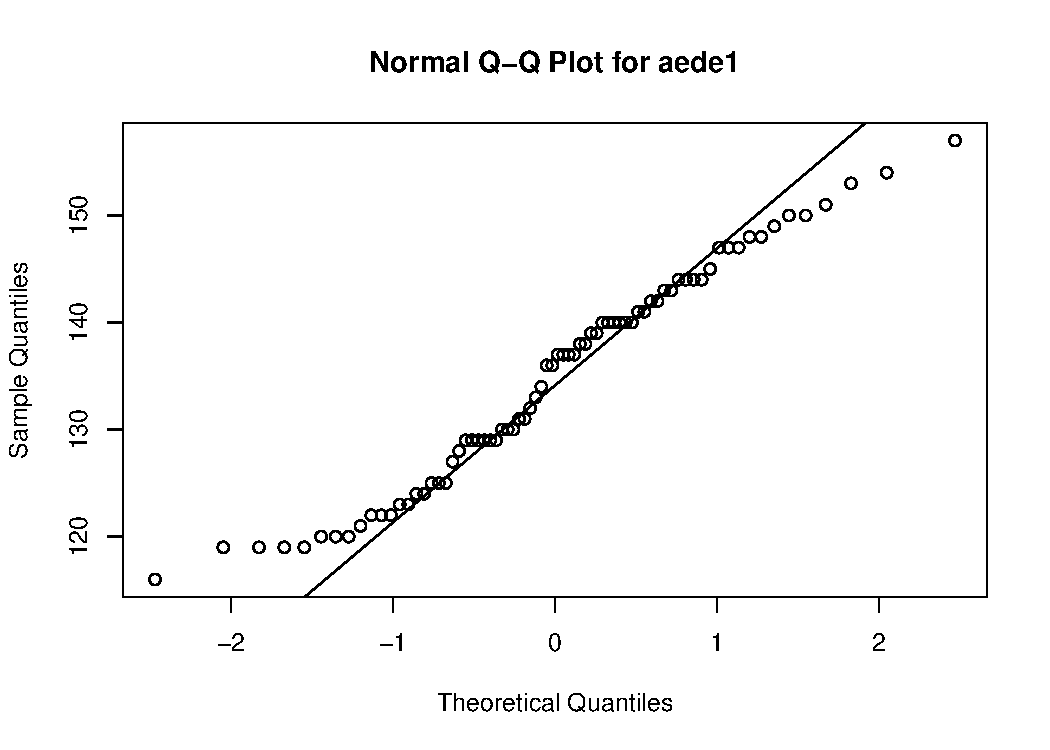
\includegraphics[width=0.8\linewidth]{multivariate_lab_hw2_files/figure-latex/unnamed-chunk-2-4} \end{center}

\begin{center}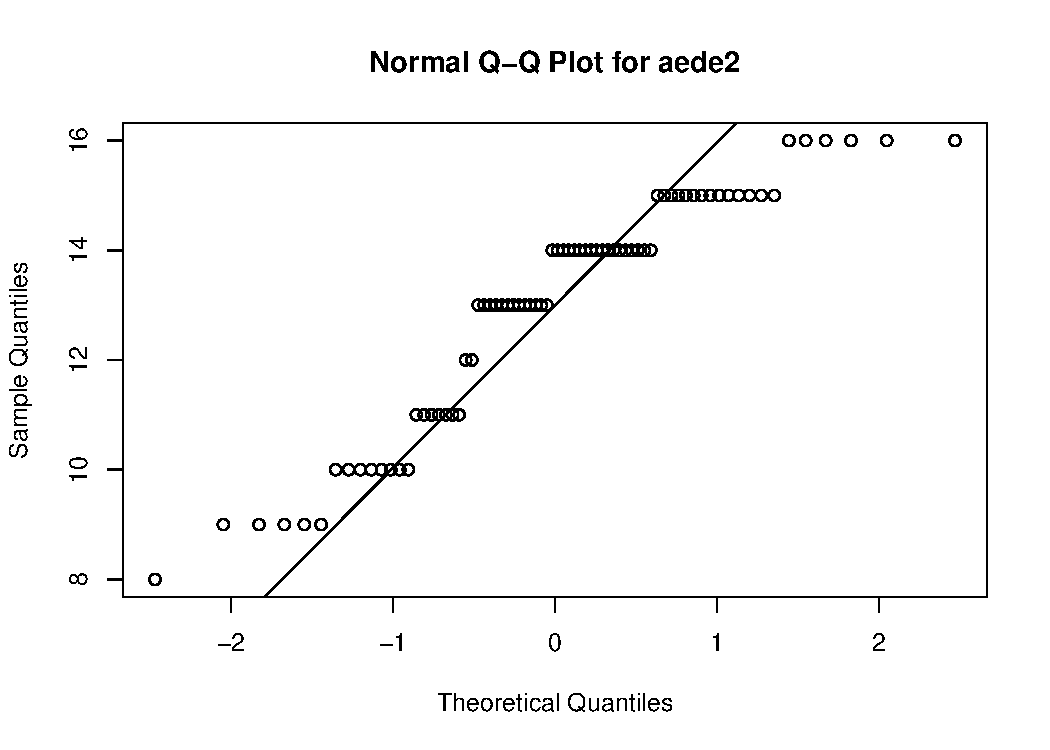
\includegraphics[width=0.8\linewidth]{multivariate_lab_hw2_files/figure-latex/unnamed-chunk-2-5} \end{center}

\begin{center}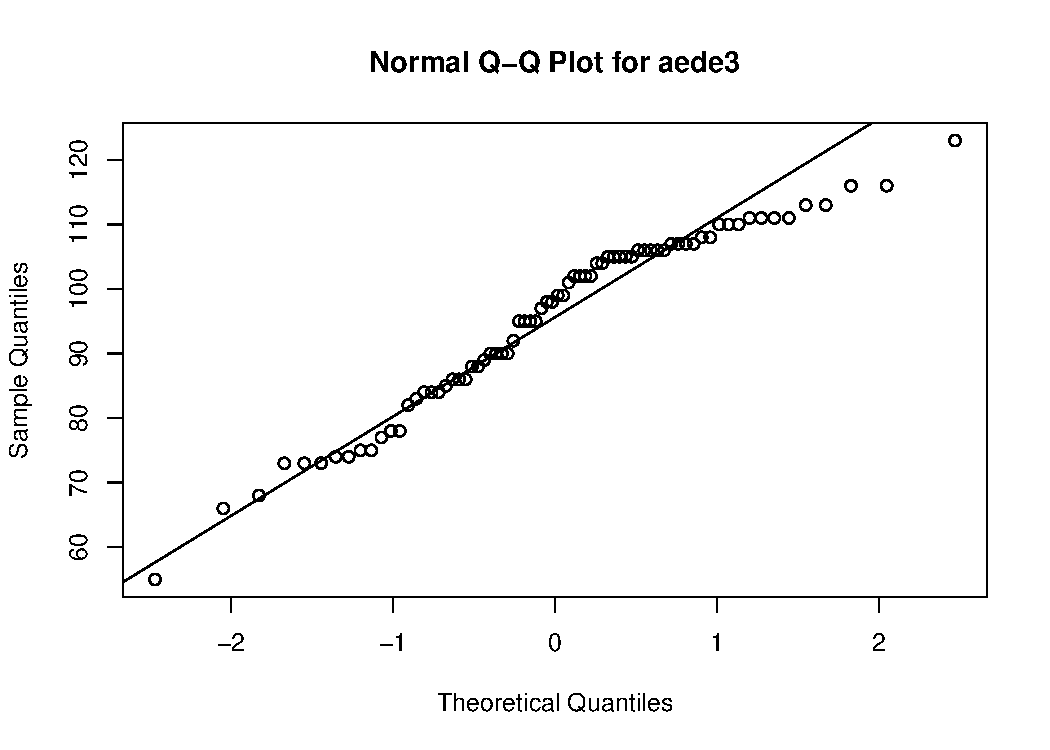
\includegraphics[width=0.8\linewidth]{multivariate_lab_hw2_files/figure-latex/unnamed-chunk-2-6} \end{center}

tars1, aede1, aede2 등에서 정규성 가정이 의심스러운 지점이 발견된다.

\subsection{Joint normality :
M-distance}\label{joint-normality-m-distance}

\begin{Shaded}
\begin{Highlighting}[]
\NormalTok{Xc }\OtherTok{\textless{}{-}} \FunctionTok{scale}\NormalTok{(}\FunctionTok{as.matrix}\NormalTok{(flea[, }\DecValTok{2}\SpecialCharTok{:}\DecValTok{7}\NormalTok{]), }\AttributeTok{scale=}\ConstantTok{FALSE}\NormalTok{)}
\NormalTok{S }\OtherTok{\textless{}{-}} \FunctionTok{t}\NormalTok{(Xc) }\SpecialCharTok{\%*\%}\NormalTok{ Xc}

\NormalTok{Mdist }\OtherTok{\textless{}{-}} \FunctionTok{sqrt}\NormalTok{(}\FunctionTok{diag}\NormalTok{(Xc }\SpecialCharTok{\%*\%} \FunctionTok{solve}\NormalTok{(S) }\SpecialCharTok{\%*\%} \FunctionTok{t}\NormalTok{(Xc))) }
\FunctionTok{qqplot}\NormalTok{(}\FunctionTok{qchisq}\NormalTok{(}\FunctionTok{ppoints}\NormalTok{(}\DecValTok{100}\NormalTok{), }\AttributeTok{df=}\DecValTok{6}\NormalTok{), Mdist}\SpecialCharTok{\^{}}\DecValTok{2}\NormalTok{)}
\end{Highlighting}
\end{Shaded}

\begin{center}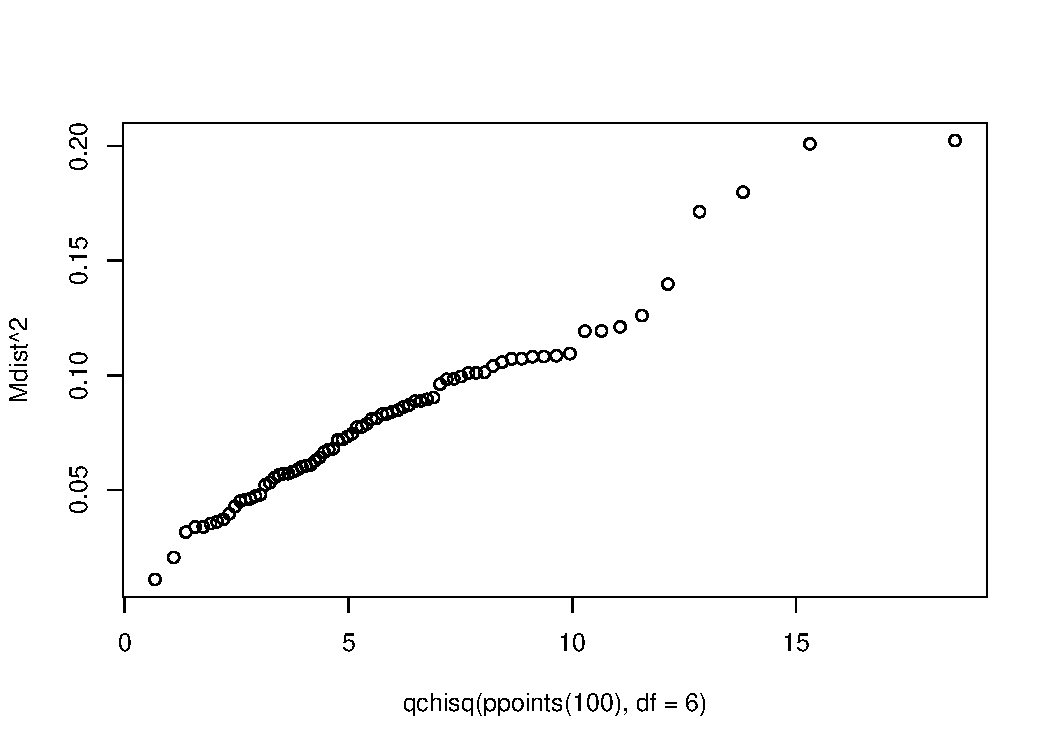
\includegraphics[width=0.8\linewidth]{multivariate_lab_hw2_files/figure-latex/unnamed-chunk-3-1} \end{center}

별로 직선에 가까워 보이지 않는다\ldots{} 정규성 가정에 의심을 품고
검정을 진행해야 할 수 있다.

\begin{center}\rule{0.5\linewidth}{0.5pt}\end{center}

\section{3}\label{section-2}

Manually compute the Between-variance matrix B from ``mean\_vectors''.
Check whether your result is equal to B = Tot - W above.

\subsection{Calculate B from B = total variance -
W}\label{calculate-b-from-b-total-variance---w}

\begin{Shaded}
\begin{Highlighting}[]
\NormalTok{n }\OtherTok{\textless{}{-}} \FunctionTok{nrow}\NormalTok{(flea)}
\NormalTok{p }\OtherTok{\textless{}{-}} \FunctionTok{ncol}\NormalTok{(flea) }\SpecialCharTok{{-}} \DecValTok{1}
\NormalTok{G }\OtherTok{\textless{}{-}} \FunctionTok{unique}\NormalTok{(flea}\SpecialCharTok{$}\NormalTok{species)}

\CommentTok{\# calculate W : within sum of squares}
\NormalTok{W }\OtherTok{\textless{}{-}} \FunctionTok{matrix}\NormalTok{(}\DecValTok{0}\NormalTok{, }\AttributeTok{nrow =}\NormalTok{ p, }\AttributeTok{ncol =}\NormalTok{ p)}
\ControlFlowTok{for}\NormalTok{ (g }\ControlFlowTok{in}\NormalTok{ G) \{}
\NormalTok{  gData }\OtherTok{\textless{}{-}} \FunctionTok{as.matrix}\NormalTok{(flea[flea}\SpecialCharTok{$}\NormalTok{species }\SpecialCharTok{==}\NormalTok{ g, }\DecValTok{2}\SpecialCharTok{:}\DecValTok{7}\NormalTok{]) }
\NormalTok{  W }\OtherTok{\textless{}{-}}\NormalTok{ W }\SpecialCharTok{+} \FunctionTok{t}\NormalTok{(}\FunctionTok{scale}\NormalTok{(gData, }\AttributeTok{scale=}\ConstantTok{FALSE}\NormalTok{)) }\SpecialCharTok{\%*\%}\NormalTok{ (}\FunctionTok{scale}\NormalTok{(gData, }\AttributeTok{scale=}\ConstantTok{FALSE}\NormalTok{))}

\NormalTok{\}}
\NormalTok{Sp }\OtherTok{\textless{}{-}}\NormalTok{ W }\SpecialCharTok{/}\NormalTok{ (n }\SpecialCharTok{{-}} \FunctionTok{length}\NormalTok{(G)) }\CommentTok{\# pooled variance}

\CommentTok{\# total variance = W + B = within variance + residual variance}
\NormalTok{Total\_variance }\OtherTok{\textless{}{-}} \FunctionTok{cov}\NormalTok{(flea[,}\DecValTok{2}\SpecialCharTok{:}\DecValTok{7}\NormalTok{]) }\SpecialCharTok{*}\NormalTok{ (n}\DecValTok{{-}1}\NormalTok{) }\CommentTok{\# total variance}
\NormalTok{B }\OtherTok{\textless{}{-}}\NormalTok{ Total\_variance }\SpecialCharTok{{-}}\NormalTok{ W }\CommentTok{\# treatment variance}
\end{Highlighting}
\end{Shaded}

\subsection{calculate B directly from mean
vector}\label{calculate-b-directly-from-mean-vector}

\begin{Shaded}
\begin{Highlighting}[]
\NormalTok{tmean }\OtherTok{\textless{}{-}} \FunctionTok{c}\NormalTok{(}\FunctionTok{colMeans}\NormalTok{(flea[, }\DecValTok{2}\SpecialCharTok{:}\DecValTok{7}\NormalTok{]))}
\NormalTok{B\_new }\OtherTok{\textless{}{-}} \FunctionTok{matrix}\NormalTok{(}\DecValTok{0}\NormalTok{, }\AttributeTok{nrow =}\NormalTok{ p, }\AttributeTok{ncol =}\NormalTok{ p)}

\ControlFlowTok{for}\NormalTok{ (g }\ControlFlowTok{in}\NormalTok{ G) \{}
\NormalTok{  gData }\OtherTok{\textless{}{-}} \FunctionTok{as.matrix}\NormalTok{(flea[flea}\SpecialCharTok{$}\NormalTok{species }\SpecialCharTok{==}\NormalTok{ g, }\DecValTok{2}\SpecialCharTok{:}\DecValTok{7}\NormalTok{]) }
\NormalTok{  n\_g }\OtherTok{\textless{}{-}} \FunctionTok{nrow}\NormalTok{(gData)}
\NormalTok{  gmean }\OtherTok{\textless{}{-}} \FunctionTok{c}\NormalTok{(}\FunctionTok{colMeans}\NormalTok{(gData))}
\NormalTok{  B\_new }\OtherTok{\textless{}{-}}\NormalTok{ B\_new }\SpecialCharTok{+}\NormalTok{ n\_g }\SpecialCharTok{*} \FunctionTok{outer}\NormalTok{(gmean}\SpecialCharTok{{-}}\NormalTok{tmean, gmean}\SpecialCharTok{{-}}\NormalTok{tmean)}
\NormalTok{\}}
\end{Highlighting}
\end{Shaded}

\subsection{B(tot - W)와 B\_new(직접 계산)
비교}\label{btot---wuxc640-b_newuxc9c1uxc811-uxacc4uxc0b0-uxbe44uxad50}

\begin{Shaded}
\begin{Highlighting}[]
\NormalTok{B}
\end{Highlighting}
\end{Shaded}

\begin{verbatim}
##            tars1      tars2       head      aede1      aede2      aede3
## tars1  51704.448 -3690.5371 -2045.2449 -9059.6608  3581.9018 -19048.520
## tars2  -3690.537  1367.3336   349.0408  2899.9057  -127.7174   3472.460
## head   -2045.245   349.0408   118.2533   772.8361  -118.1519   1142.130
## aede1  -9059.661  2899.9057   772.8361  6186.6528  -366.4563   7650.271
## aede2   3581.902  -127.7174  -118.1519  -366.4563   262.9717  -1074.726
## aede3 -19048.520  3472.4598  1142.1297  7650.2713 -1074.7255  11061.516
\end{verbatim}

\begin{Shaded}
\begin{Highlighting}[]
\NormalTok{B\_new}
\end{Highlighting}
\end{Shaded}

\begin{verbatim}
##            tars1      tars2       head      aede1      aede2      aede3
## tars1  51704.448 -3690.5371 -2045.2449 -9059.6608  3581.9018 -19048.520
## tars2  -3690.537  1367.3336   349.0408  2899.9057  -127.7174   3472.460
## head   -2045.245   349.0408   118.2533   772.8361  -118.1519   1142.130
## aede1  -9059.661  2899.9057   772.8361  6186.6528  -366.4563   7650.271
## aede2   3581.902  -127.7174  -118.1519  -366.4563   262.9717  -1074.726
## aede3 -19048.520  3472.4598  1142.1297  7650.2713 -1074.7255  11061.516
\end{verbatim}

\begin{Shaded}
\begin{Highlighting}[]
\FunctionTok{all.equal}\NormalTok{(B, B\_new)}
\end{Highlighting}
\end{Shaded}

\begin{verbatim}
## [1] TRUE
\end{verbatim}

두 행렬을 비교하면 서로 같음을 확인할 수 있다.

\begin{center}\rule{0.5\linewidth}{0.5pt}\end{center}

\section{4}\label{section-3}

How many positive eigenvalues should you see in the above?

우선, 모델을 먼저 적합한다.

\begin{Shaded}
\begin{Highlighting}[]
\NormalTok{result\_m }\OtherTok{\textless{}{-}} \FunctionTok{manova}\NormalTok{(}\FunctionTok{as.matrix}\NormalTok{(flea[,}\DecValTok{2}\SpecialCharTok{:}\DecValTok{7}\NormalTok{]) }\SpecialCharTok{\textasciitilde{}}\NormalTok{ species, }\AttributeTok{data =}\NormalTok{ flea)}
\NormalTok{result\_p }\OtherTok{\textless{}{-}} \FunctionTok{summary}\NormalTok{(result\_m, }\AttributeTok{test =} \StringTok{"Pillai"}\NormalTok{) }\CommentTok{\# default.}
\NormalTok{result\_p}
\end{Highlighting}
\end{Shaded}

\begin{verbatim}
##           Df Pillai approx F num Df den Df    Pr(>F)    
## species    2 1.7421   75.413     12    134 < 2.2e-16 ***
## Residuals 71                                            
## ---
## Signif. codes:  0 '***' 0.001 '**' 0.01 '*' 0.05 '.' 0.1 ' ' 1
\end{verbatim}

\begin{Shaded}
\begin{Highlighting}[]
\NormalTok{result\_w }\OtherTok{\textless{}{-}} \FunctionTok{summary}\NormalTok{(result\_m, }\AttributeTok{test =} \StringTok{"Wilks"}\NormalTok{)}
\NormalTok{result\_w}
\end{Highlighting}
\end{Shaded}

\begin{verbatim}
##           Df  Wilks approx F num Df den Df    Pr(>F)    
## species    2 0.0109   94.359     12    132 < 2.2e-16 ***
## Residuals 71                                            
## ---
## Signif. codes:  0 '***' 0.001 '**' 0.01 '*' 0.05 '.' 0.1 ' ' 1
\end{verbatim}

\begin{Shaded}
\begin{Highlighting}[]
\NormalTok{result\_h }\OtherTok{\textless{}{-}} \FunctionTok{summary}\NormalTok{(result\_m, }\AttributeTok{test =} \StringTok{"Hotelling{-}Lawley"}\NormalTok{)}
\NormalTok{result\_r }\OtherTok{\textless{}{-}} \FunctionTok{summary}\NormalTok{(result\_m, }\AttributeTok{test =} \StringTok{"Roy"}\NormalTok{)}
\end{Highlighting}
\end{Shaded}

다음으로, 비교 대상이 되는 행렬들을 확인하자. 부동소수점 오차를 고려하여
\texttt{all.equal()} 함수를 사용하여 B, W와 MANOVA 결과의 행렬들을
비교한다.

\begin{Shaded}
\begin{Highlighting}[]
\FunctionTok{all.equal}\NormalTok{(result\_p}\SpecialCharTok{$}\NormalTok{SS}\SpecialCharTok{$}\NormalTok{species, B)}
\end{Highlighting}
\end{Shaded}

\begin{verbatim}
## [1] TRUE
\end{verbatim}

\begin{Shaded}
\begin{Highlighting}[]
\FunctionTok{all.equal}\NormalTok{(result\_p}\SpecialCharTok{$}\NormalTok{SS}\SpecialCharTok{$}\NormalTok{Residuals, W)}
\end{Highlighting}
\end{Shaded}

\begin{verbatim}
## [1] TRUE
\end{verbatim}

\begin{Shaded}
\begin{Highlighting}[]
\FunctionTok{all.equal}\NormalTok{(result\_w}\SpecialCharTok{$}\NormalTok{SS}\SpecialCharTok{$}\NormalTok{species, B)}
\end{Highlighting}
\end{Shaded}

\begin{verbatim}
## [1] TRUE
\end{verbatim}

\begin{Shaded}
\begin{Highlighting}[]
\FunctionTok{all.equal}\NormalTok{(result\_w}\SpecialCharTok{$}\NormalTok{SS}\SpecialCharTok{$}\NormalTok{Residuals, W)}
\end{Highlighting}
\end{Shaded}

\begin{verbatim}
## [1] TRUE
\end{verbatim}

비교 결과, 앞서 계산했던 B, W와 \texttt{manova()} 함수를 활용해 계산한
B, W가 서로 같음을 확인할 수 있다. 그렇다면, 총 몇 개의 eignevalues가
양수여야 하는가? 당연히 B와 W 모두 적어도 Non-Negative matrix이므로 B, W
각각 6개씩 총 12개의 고윳값이 nonnegative여야 한다. \(W^{-1}*B\) 역시
nonnegative여야 하는데, 이를 포함하면 6개가 추가되어 18개이다. 그런데!

\begin{Shaded}
\begin{Highlighting}[]
\FunctionTok{sum}\NormalTok{(}\FunctionTok{eigen}\NormalTok{(B)}\SpecialCharTok{$}\NormalTok{values }\SpecialCharTok{\textgreater{}} \DecValTok{0}\NormalTok{)}
\end{Highlighting}
\end{Shaded}

\begin{verbatim}
## [1] 4
\end{verbatim}

\begin{Shaded}
\begin{Highlighting}[]
\FunctionTok{sum}\NormalTok{(}\FunctionTok{eigen}\NormalTok{(W)}\SpecialCharTok{$}\NormalTok{values }\SpecialCharTok{\textgreater{}} \DecValTok{0}\NormalTok{)}
\end{Highlighting}
\end{Shaded}

\begin{verbatim}
## [1] 6
\end{verbatim}

B에서 고윳값이 음수이다. 왜인가? 수치선형대수상의 오차 때문이다.
특성다항식의 풀이는 오차가 꽤나 발생하는 풀이로, 특히 B와 같이 행렬을
구성하는 각 원소의 사이즈가 큰 경우에는 이와 같이 음수가 될 수 있다.

\begin{center}\rule{0.5\linewidth}{0.5pt}\end{center}

\section{5}\label{section-4}

All of the MANOVA Tests above are not valid if normality is not assumed.
For such cases, one may use permutation-based test. Inspect the
following lines and report your conclusion.

순열 검정의 귀무가설은 'null hypothesis of exchangeability'로, 집단 간
차이가 없다면 샘플 간 교환을 수행하였을 때(순열 함수를 적용하였을 때의
데이터)의 검정통계량이 원래 데이터의 통계량과 큰 차이가 없을 것이라는
것이다.

\begin{Shaded}
\begin{Highlighting}[]
\CommentTok{\#library(purrr)}
\FunctionTok{library}\NormalTok{(modelr)}
\NormalTok{perms }\OtherTok{\textless{}{-}} \FunctionTok{permute}\NormalTok{(flea, }\DecValTok{1000}\NormalTok{, species)}
\NormalTok{permuted\_Wilk }\OtherTok{\textless{}{-}} \FunctionTok{map}\NormalTok{(perms}\SpecialCharTok{$}\NormalTok{perm,}
              \SpecialCharTok{\textasciitilde{}} \FunctionTok{summary}\NormalTok{(}\FunctionTok{manova}\NormalTok{(}\FunctionTok{as.matrix}\NormalTok{(flea[,}\DecValTok{2}\SpecialCharTok{:}\DecValTok{7}\NormalTok{]) }\SpecialCharTok{\textasciitilde{}}\NormalTok{ species, }\AttributeTok{data =}\NormalTok{ .),}\AttributeTok{test =} \StringTok{"Wilks"}\NormalTok{)}\SpecialCharTok{$}\NormalTok{stats[}\DecValTok{3}\NormalTok{])}
\NormalTok{permuted\_Wilk }\OtherTok{\textless{}{-}} \FunctionTok{unlist}\NormalTok{(permuted\_Wilk)}

\NormalTok{actual\_Wilk }\OtherTok{\textless{}{-}}\NormalTok{ result\_w}\SpecialCharTok{$}\NormalTok{stats[}\DecValTok{3}\NormalTok{] }
\NormalTok{p\_value }\OtherTok{\textless{}{-}} \FunctionTok{sum}\NormalTok{(permuted\_Wilk }\SpecialCharTok{\textless{}=}\NormalTok{ actual\_Wilk)}\SpecialCharTok{/}\DecValTok{1000}
\NormalTok{p\_value}
\end{Highlighting}
\end{Shaded}

\begin{verbatim}
## [1] 0
\end{verbatim}

\begin{Shaded}
\begin{Highlighting}[]
\FunctionTok{hist}\NormalTok{(permuted\_Wilk)}
\end{Highlighting}
\end{Shaded}

\begin{center}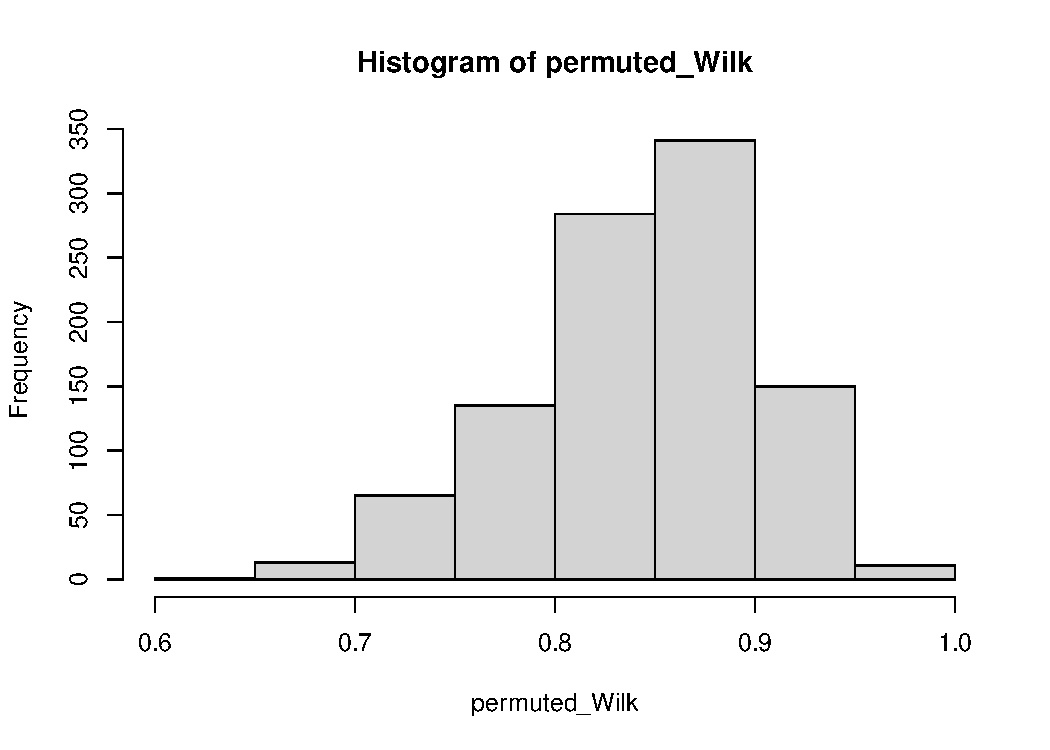
\includegraphics[width=0.8\linewidth]{multivariate_lab_hw2_files/figure-latex/unnamed-chunk-10-1} \end{center}

\texttt{library(purrr)} : \texttt{map()} 함수를 쓰기 위해 사용하였다.
위에서 \texttt{tidyverse} 라이브러리를 로드하였으므로 해당 블록에서는
주석 처리하였다.

\texttt{library(modelr)} : \texttt{permute()} 함수를 통해 순열 검정을
수행하기 위해 로드하였다.

\texttt{perms} : \texttt{permute()} 함수를 통해 순열 검정을 위한 데이터
섞기를 수행하였다. flea는 data, 1000은 만들 총 순열의 개수, species는
permute할 칼럼이다. 예시 코드의 n = 100과 달리 n = 1000으로 수행하였다.

\texttt{map()} + \texttt{unlist()} : map()은 dataframe 등에 적용되어
list 자료형을 결과로 return하는 함수이다. 구체적으로, map() 함수는
dataframe의 각 원소마다 특정한 함수를 적용하고, 그 함수의 결과를 list로
반환한다. 해당 코드에서는 \texttt{perms} list에 있는 각 계승마다
manova를 적용하고, 그로부터 Wilk 검정통계랑을 계산하여 그 값을 리스트로
반환한다. 이후 \texttt{unlist()} 함수를 적용하는 것은 리스트를 다시
values sequence로 변환한 것이다.

\texttt{actual\_Wilk} : 앞서 Wilk 검정통계량을 계산한 모델이 있으므로
이로부터 실제 검정통계량과 비교하여 p-value를 계산하기 위해 추가하였다.

히스토그램에 별도의 p-value를 표기하지 않았다. 0에 가까운 값이므로
표기하기 위해 축을 변형하는 것이 축을 오히려 왜곡하여 오도할 것으로
판단하였다.

p\_value \textless{} 0.0001 수준의 매우 작은 값이므로 그룹 간 차이가
있다고 판단할 수 있다.

\end{document}
